TODO Heuristik-Blah

\subsection{Spring Embedder}

Spring Embedder sind eine Familie von Algorithmen zum Zeichnen von Graphen. Diese Algorithmen basieren im Allgemeinen darauf, dass ein physikalisches Modell simuliert wird, bei dem Kräfte auf die einzelnen Knoten wirken, die diese verschieben. Spring Embedder sind weit verbreitet, gut verstanden und recht flexibel\cite{kobourov2012spring}, sodass es naheliegend ist, diese als Möglichkeit in Betracht zu ziehen.

Wenn wir davon ausgehen, dass im gelayouteten Graphen nur die Kantenlängen (und nicht die Richtung der Kanten) das Layout bestimmen, dann ist der Term \ref{eqn:opt:basic} trivial in einen Spring Embedder umzusetzen. Dies wäre insbesondere geeignet, falls der Graph eine hohe Steifigkeit aufweist, da in diesem Fall die Kantenlängen allein das Layout des Graphen festlegen.\footnote{Dies ist nicht ganz korrekt: Es können mehrere unterschiedliche geometrische Einbettungen mit denselben Kantenlängen existieren, z.B. indem Dreiecke umgeklappt werden. Da ein Spring Embedder allerdings nur kleine, inkrementelle Änderungen der Einbettung vornimmt, ist dies hier nicht relevant.}

\begin{figure}
	\centering
	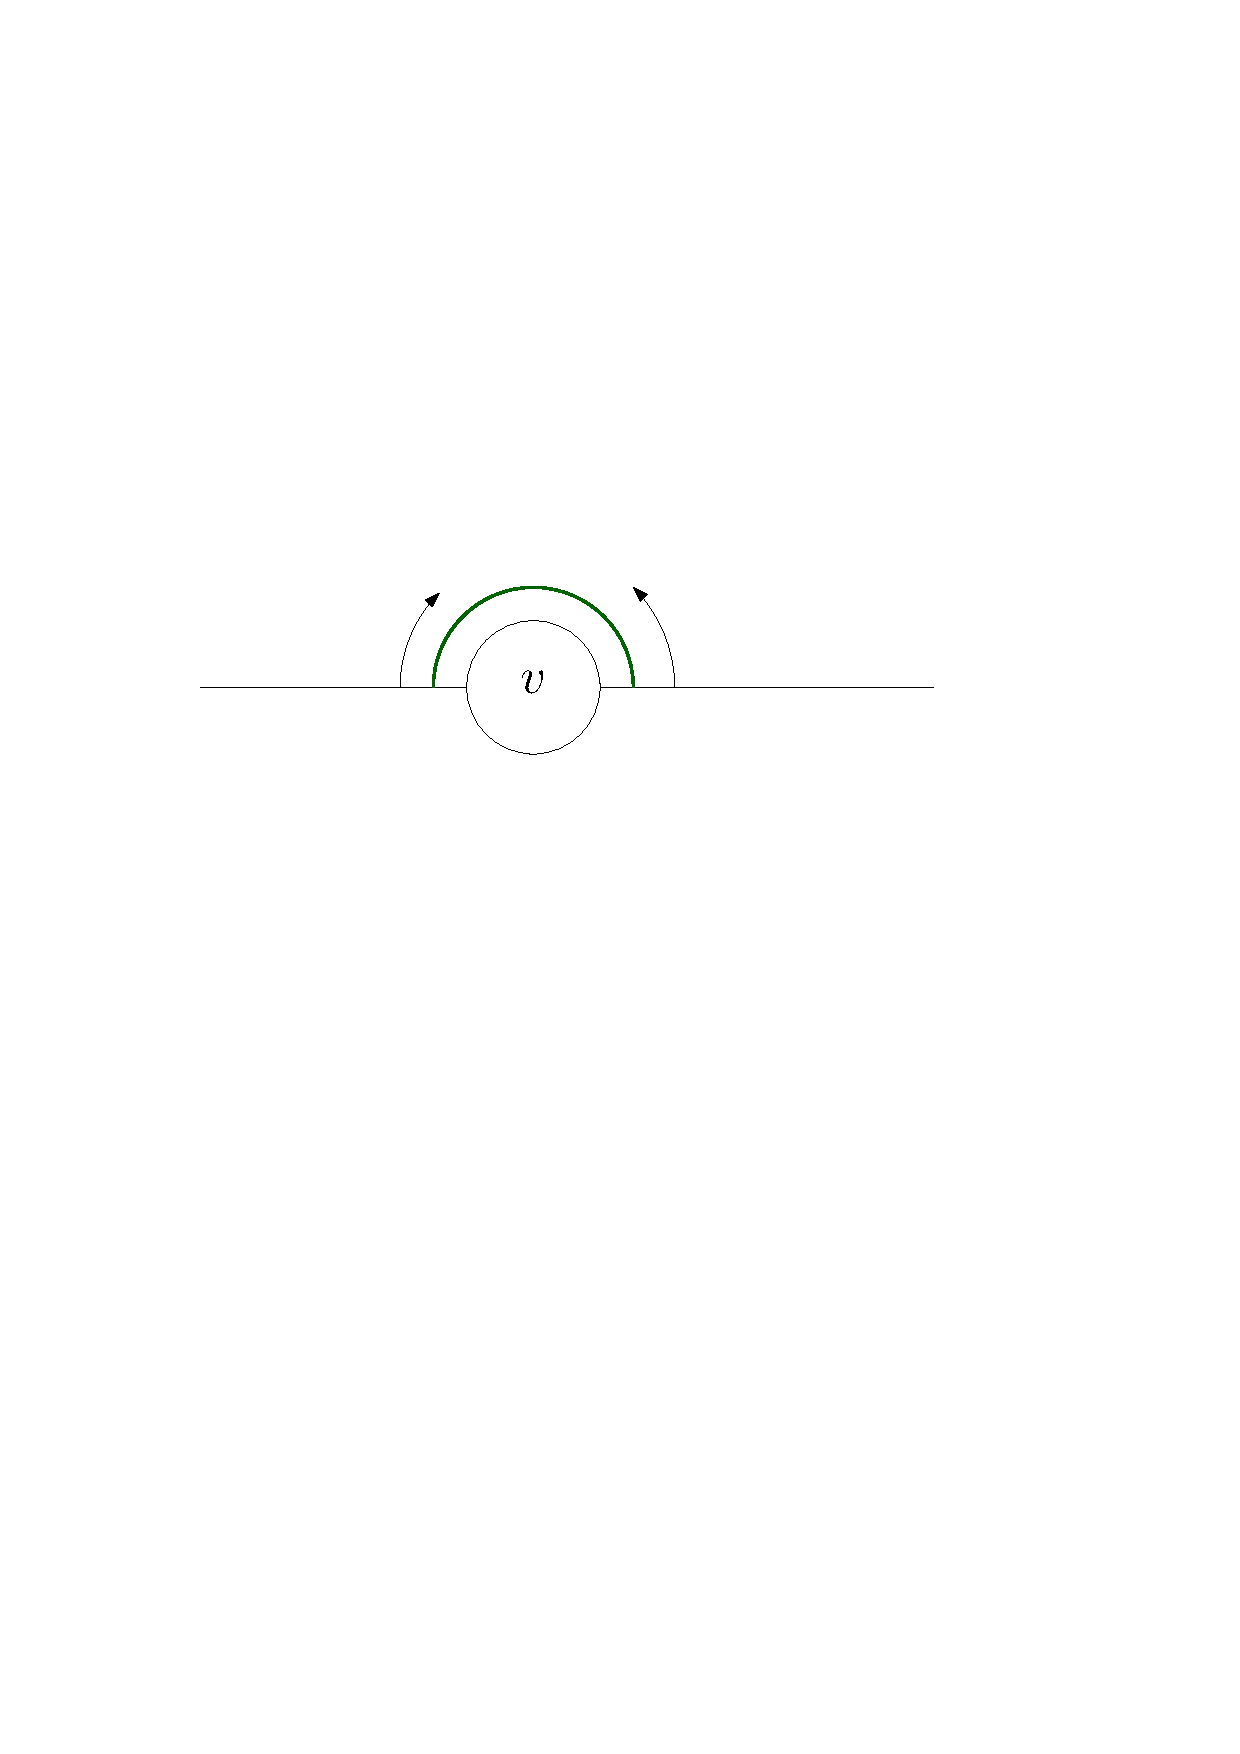
\includegraphics{figures/orbitalspring.pdf}
	\caption{Eine orbitale Feder}
	\label{fig:orbitalspring}
\end{figure}

Leider sind Argumentkarten vergleichsweise dünn besetzte Graphen, und daher ist eine geringe Steifigkeit anzunehmen. Um hier zu dem von Term \ref{eqn:opt:basic} gewünschten Ergebnis zu kommen, wäre es vermutlich notwendig, zusätzlich orbitale Federn um die Knoten herum zu legen, die die Winkel der ausgehenden Kanten relativ zueinander an das gewünschte Ergebnis anzunähern. Siehe Abbildung \ref{fig:orbitalspring}. Hier zieht die grüne kreisförmige Feder die beiden aus $v$ ausgehenden Kanten zusammen. Solche kreisförmigen Federn sind beispielsweise bereits erfolgreich für Lombardi-Zeichnungen mit optimaler Winkelauflösung verwendet worden\cite{chernobelskiy2012force}, wobei hier die Kräfte den kompletten Knoten rotiert haben, statt Auswirkungen auf die adjazenten Knoten zu haben. Kreisförmige Federn zischen Kantenpaaren konnten wir in der Literatur bisher keine finden. TODO nochmal überprüfen!

\subsection{Seam Carving}

Seam Carving ist eine verbreitete Methode in der Bildbearbeitung, die von S. Avidan und A. Shamir vorgestellt wurde.\cite{avidan2007seam} Das Ziel von Seam Carving ist es, ein Bild zu verkleinern, indem Pixel weggelassen werden, ohne visuell den Eindruck einer Verzerrung zu erwecken. Hierfür verwendet Seam Carving eine Technik, die die Autoren als "`content aware"' bezeichnen: Die wegzulassenden Pixel werden als durchgänginge Streifen, die sogenannten "`Seams"', gewählt. Bei der Auswahl der Seams wird darauf geachtet, dass diese möglichst wenig durch Bereiche des Bildes verlaufen, in denen ein Weglassen störend wäre. Hierfür beschreiben die Autoren verschiedene Energiefunktionen auf den Bildern.

\begin{figure}
	\centering
	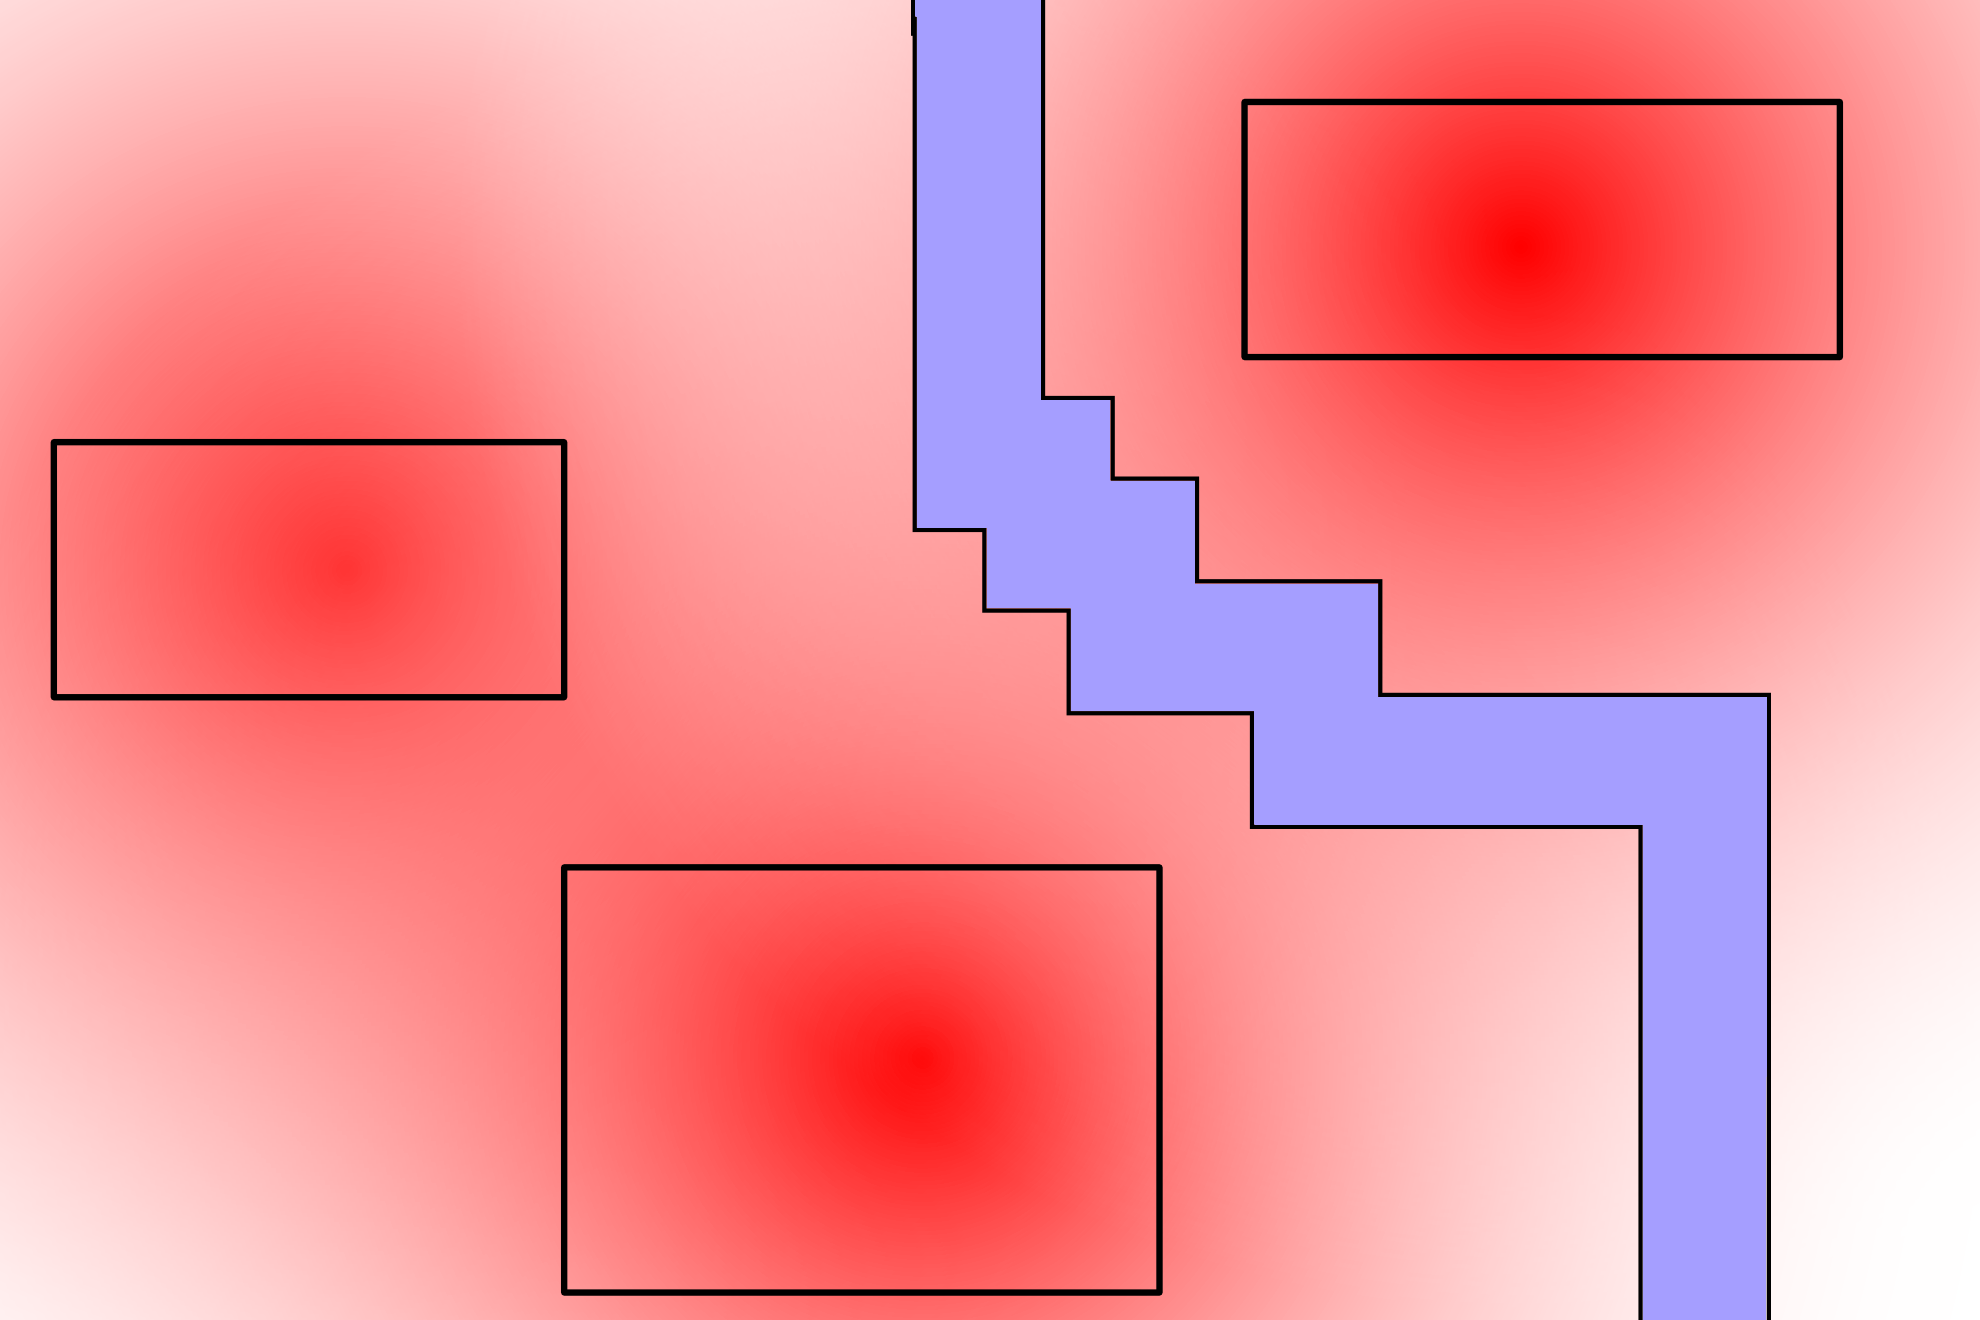
\includegraphics{figures/seamcarving.png}
	\caption{Seam Carving}
	\label{fig:seamcarving}
\end{figure}

Seam Carving hat außerdem bereits Anwendung im Bereich des Graph Drawings gefunden, beispielsweise beim Layout von Word Clouds.\cite{wu2011semantic} Das Vorgehen war hier das folgende: Ein initiales Layout verteilt die Knoten des Graphens mittels Multidimensional Scalings nach bestimmten vorgegbenen Abständen voneinander. Der überflüssige Platz wird dann mit Seam Carving entfernt. Hierbei sollten die relativen Positionen der Knoten möglichst wenig verzerrt werden. Die Autoren beschreiben hierfür die für das Seam Carving verwendete Energiefunktion als Summe der Quadrate der inversen Abstände von den Knoten. In Abbildung \ref{fig:seamcarving} ist eine solche Zeichnung mit den Energiefunktionen und einem möglichen Seam dargestellt.

Ein ähnlicher Ansatz ist auch für unser Problem denkbar. Wie in Absatz \ref{sub:problem} beschrieben, ist es immer möglich, alle Kanten einfach so lange zu skalieren, bis der neue Knoten überlappungsfrei platziert werden kann. TODO Paragraph referenzieren? Das Problem besteht hier darin, dass das gesamte Layout hierbei beliebig groß werden kann, zur Betrachtung also das Bild insgesamt verkleinert werden muss, was einer Skalierung der Knotergrößen gleichkommt. Dieses Problem könnte dadurch angegangen werden, dass das in \cite{wu2011semantic} beschriebene Verfahren ohne große Änderungen auf das Layout nach der Skalierung angewendet wird.
